\preClass{Coordinate Systems}


\videoLink{Section 3.1}{https://www.youtube.com/playlist?list=PLYHZK3b8UFw2aq4QBoSuTAkPcWN5e-afh}


\begin{enumerate}

\item  Determine if $f(x)=-4x+1$ is one-to-one both algebraically and graphically.
\begin{enumerate}

\item  Graph $f(x)=-4x+1$ and use the graph to determine if $f(x)$ is
  one-to-one.
  \sideNote{Briefly explain your reasoning and do not simply state the name of a theorem or rule.}

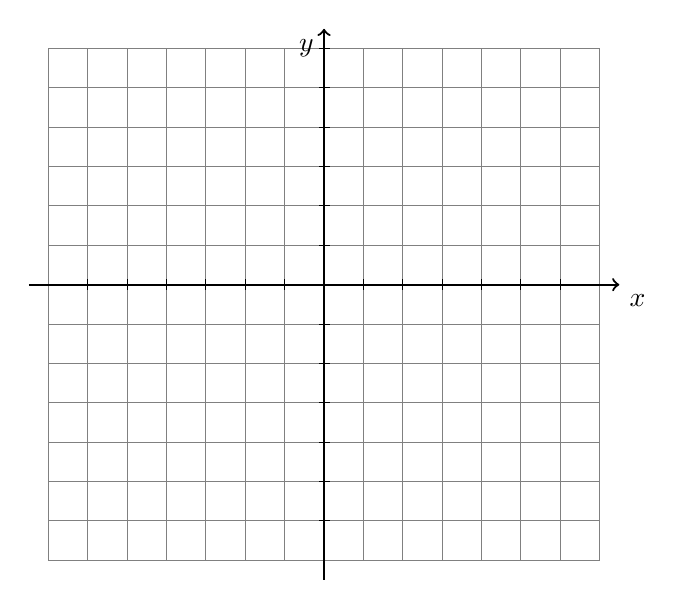
\begin{tikzpicture}[y=.5cm, x=0.5cm,font=\sffamily]
    %% ticks
    \draw[step = 1, gray] (-7,-7) grid (7,6);
    %% axis
    \draw[thick,->] (-7.5,0) -- coordinate (x axis mid) (7.5,0) node[anchor = north west] {$x$};
    \draw[thick,->] (0,-7.5) -- coordinate (y axis mid) (0,6.5) node[anchor = north east] {$y$};
    \foreach \y in {-6,-5,...,-1,1,2,...,6} {
      \draw (2pt, \y) -- (-2pt, \y);
    }
    \foreach \x in {-6,-5,...,-1,1,2,...,6} {
      \draw (\x,2pt) -- (\x,-2pt);
    }

\end{tikzpicture}

\vspace{2em}

\item  Algebraically determine if $f(x)=-4x+1$ is one-to-one.

\vfill


\end{enumerate}



\vfill
\clearpage

\item   Let $f(x)=5x+4$ and $\displaystyle g(x)=\frac{x-4}{5}$.\\
  Use the theorem on inverse functions (function composition) to
  determine whether $f$ and $g$ are inverses.  Show every step.
  
  \vfill


\item Determine the inverse function of $\displaystyle h(x)=\frac{8-x}{3}$.
  
  \vfill




\end{enumerate}



